% !TEX root = WWW.tex


\section{Introduction}
A body of work on large real-world networks  deals with the difficulties of storing them and to effectively resolve queries on them.
Compression techniques~\cite{boldi2004webgraph,boldi2011layered}, as  well as the dissemination  of these networks underlying graphs over several machines~\cite{gonzalez2012powergraph, stanton2012streaming} are some of the ideas suggested to treat this task.
An additional  approach to solve these difficulties is to disseminate the structural information of the graph to its vertices.
 Known as peer-to-peer, it  allows for an inference of the graph's local topology  using only local information stored in each vertex without using costly access to large, global data structures. 
As mentioned by   Buchegger et al.~\cite{buchegger2009peerson}  peer-to-peer  networks are particularly useful to address privacy concerns, and to ensure a high survivability rate. 

To that end, a useful tool is the notion of a \emph{labeling scheme}: an algorithm that assigns a bit string--a \emph{label}--to each vertex so that a query between any two vertices can be deduced solely from their respective labels. 
Labeling schemes are extremely well studied topic~\cite{katz2004labeling,gavoillea2004distance,brady2006compact,gavoille2007shorter,korman2007compact,Korman07,korman2007general,caminiti2008engineering,dahlgaard2014dynamic,rotbart2014evaluation,alstrup2014adjacency}, under the objective of  minimizing the \emph{maximum label size}: the maximum number of bits used in a label of any vertex. Among applications for them are   XML search engines~\cite{cohen2010labeling}, mapping services~\cite{abraham2011hub} and internet routing~\cite{krioukov2004compact}.

Adjacency labeling schemes for  numerous important graph families are by now well understood. 
general graphs  require a label size of $n/2+O(1)$~\cite{moon1965minimal, alstrup2014adjacency}, while 
trees, planar graphs, and bounded degree graphs enjoy labels of logarithmic size~\cite{Alstrup02, gavoille2007shorter, adjiashvili2014labeling}. 
To the best of our knowledge, we are the first to study adjacency labeling schemes for classes of graphs whose statistical properties--in particular their \emph{degree distribution}--more closely resemble that of real-world networks.

One class of graphs extensively used for modelling real-world networks is \emph{power-law graphs}: roughly, $n$-vertex graphs where the number of vertices of degree $k$ is proportional to $n/k^{\alpha}$ for some positive $\alpha$. Power-law graphs (also called scale-free graphs in the literature) have been used, e.g., to model the Internet AS-level graph \cite{DBLP:journals/ton/SiganosFFF03,DBLP:conf/podc/AkellaCKS03}, and many other types of network (see, e.g., \cite{mitzenmacher2004brief,clauset2009power} for overviews). 
The adequacy of fit of power-law graph models to actual data, as well as the empirical correctness of the conjectured mechanisms giving rise to power-law behaviour, have been subject to criticism (see, e.g., \cite{DBLP:journals/jacm/AchlioptasCKM09,clauset2009power}). 
In spite of such criticism, and because their degree distribution affords a reasonable approximation of the degree distribution of many networks, the class of power-law graphs remains a popular tool in network modelling whose statistical behaviour is well-understood: e.g., for power-law graphs with $2<\alpha<3$, the range most often seen in the modelling of real-world networks \cite{clauset2009power}, it is known that with high probability the average distance between any two vertices is  $O(\log \log n)$, the diameter is $O(\log n)$ and there exists a dense subgraph of $n^{c/\log \log n}$ vertices~\cite{chung2004average}. 

Routing labeling schemes for power-law graphs  have been investigated by Brady and Cowen~\cite{brady2006compact}, and by Chen et al.~\cite{chen2012compact}. Labeling schemes for other properties than adjacency have been investigated for various classes of graphs, e.g., distance~\cite{gavoillea2004distance}, and flow~\cite{katz2004labeling}. 
Dynamic labeling schemes were studied by Korman and Peleg~\cite{korman2007compact,Korman07,korman2007general} and recently by Dahlgaard et. al~\cite{dahlgaard2014dynamic}.
Experimental evaluation for some labeling schemes for various properties on general graphs have been performed by Caminiti et.~al~\cite{caminiti2008engineering}, Fischer~\cite{fischer2009short} and Rotbart et.~al~\cite{rotbart2014evaluation}.


\subsection{Our contribution}
For the family of power-law graphs we contribute:
\paragraph{An  $O(\sqrt[\alpha] n (\log n)^{1 - 1/\alpha})$ adjacency labeling scheme}
The scheme is based on two ideas:
(i) a labeling \emph{strategy} that  partitions the vertices of $G$ into high (``fat'') and low degree (``thin'') vertices based on a threshold degree, and (ii) a threshold \emph{prediction} that depends only on the coefficient $\alpha$ of a power-law curve fitted to the degree distribution of $G$. 
Real-world power-law graphs rarely exceed  $~10^{10}$ vertices, implying a label size of at most  ${10^{5}}$ bits, well within the processing capabilities of current hardware. 
Our  scheme may be appealing in practice,  both due  to its simplicity and the reasonable size of its labels.
Using the same ideas, we get an  asymptotically near-tight  $O(\sqrt{n \log n})$ adjacency labeling scheme for sparse graphs.

\paragraph{A lower bound of $\Omega(\sqrt[\alpha]{n})$ for any adjacency labeling scheme}
To this end we define a  restrictive subclass of power-law graphs and show that it is contained in the bigger class we study for the upper bound; we show that this class requires label size $\Omega(\sqrt[\alpha]{n})$ for $n$-vertex graphs.
This lower bound shows that our upper bound above is asymptotically  optimal, bar a $(\log n)^{1 - 1/\alpha}$ factor.
By the connections between adjacency labeling schemes and universal graphs, we also obtain upper and lower bounds for induced universal graphs for power-law graphs. 

\paragraph{An $o(n)$ distance labeling scheme}
Using similar strategy to the adjacency labeling scheme, and a small modification, we get this reult.


\paragraph{An experimental investigation  of our labeling scheme}
Using both real-world (23K-325K vertices) and synthetic (300K-1M vertices) data sets, we observe that:
(i) Our threshold \emph{prediction} performs close to optimal when using the labeling \emph{strategy} above. 
(ii) our labeling scheme achieves maximum label size several orders of magnitude smaller than the state-of-the-art labeling schemes for more general graph families.

Lastly, we mention that our study also contributes to    the graph-theory related concept of induced universal graphs. 
Given a  graph family of $n$ node graphs  $\mathcal{F}$, we look for the smallest  graph $G$ that contain all $\mathcal{F}$ as  induced sub-graphs.
A tight connection between this concept and adjacency labeling schemes was established in~\cite{Kannan92} which implies that  our labeling scheme and lower bound have implications to this field.

\begin{figure}
\centering
\subfloat[]{
    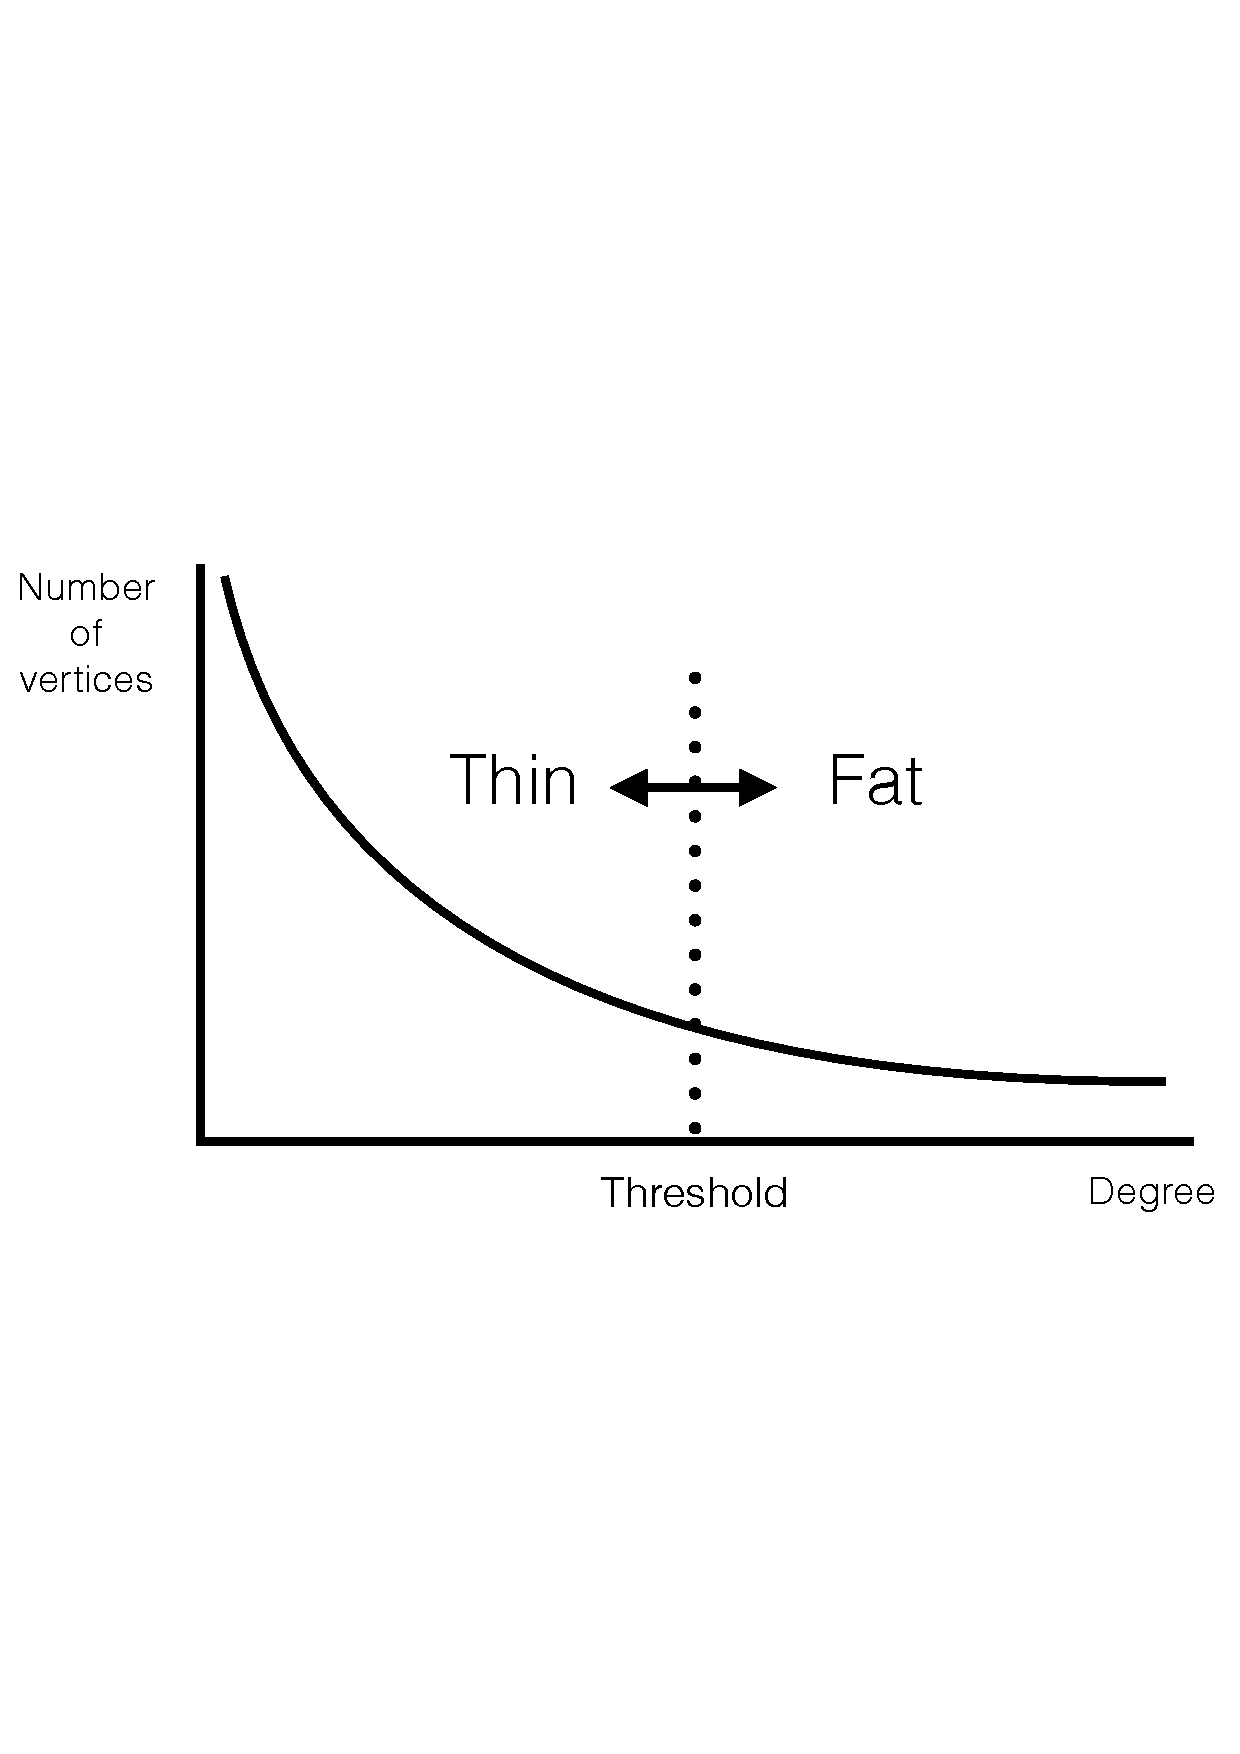
\includegraphics[width=0.23\textwidth]{Figures/Principle1.pdf}
    \label{f:principle1}
}
\subfloat[]{
    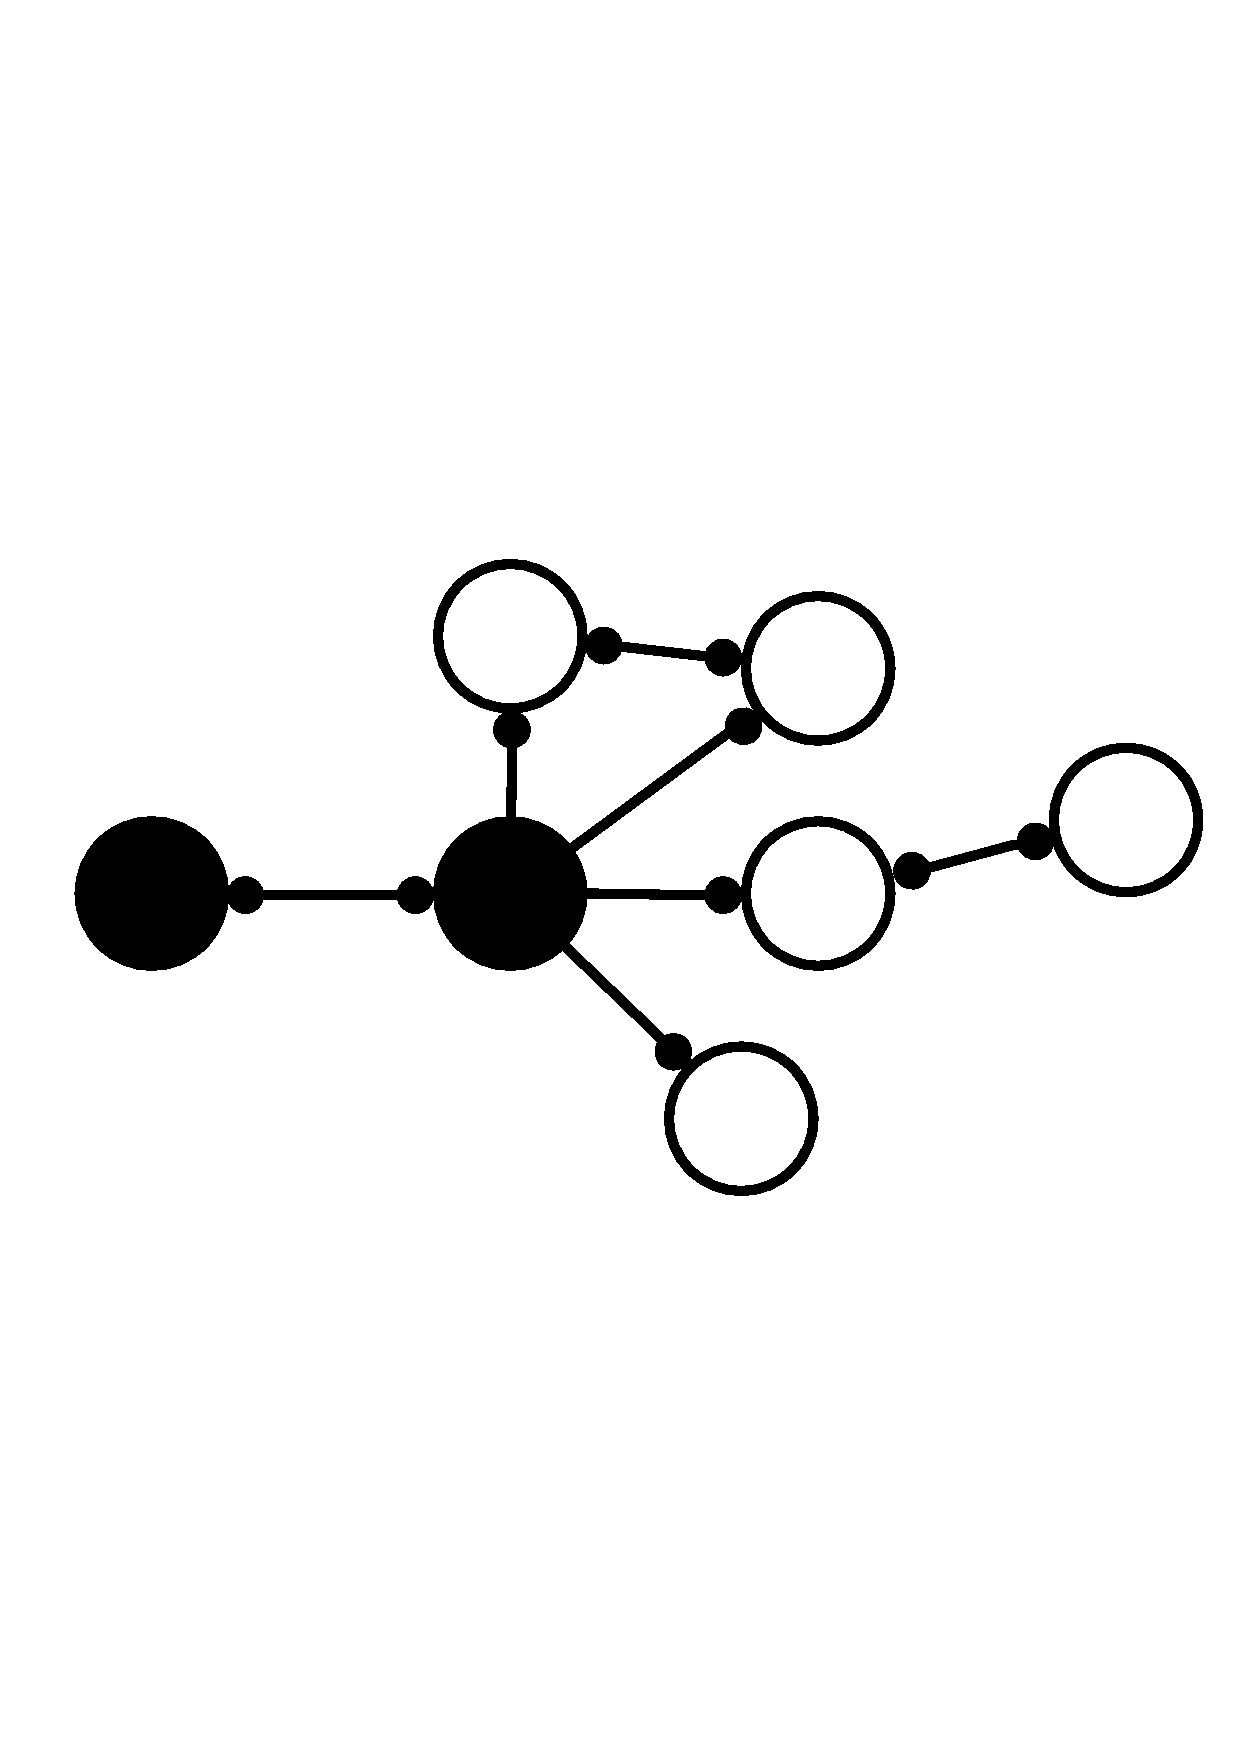
\includegraphics[width=0.23\textwidth]{Figures/Principle2.pdf}
    \label{f:principle2}
}%(
\caption{Two illustrations of the main idea. Figure (a) demonstrates the threshold assignment, figure (b) demonstrates the label assignment, in which fat (black) nodes do not store adjacency to thin (white) nodes.}
\end{figure}





